\documentclass[../rapport_MVEX01-11-05]{subfiles}
\begin{document}

\section{Klassificering av hudfärg och urskiljning av händer}
Både vår sannolikhetsfördelning för icke-hudfärg och motsvarande
fördelning från \citeasnoun{Elmezain08} har väldigt liten varians,
d.v.s. diagonalelementen i kovariansmatrisen är små. För att ge en bra
hudidentifiering bör denna varians vara stor, annars klassas allt
''bortom'' hudfärg (rödaktiga färger) som hud.
Detta kan inses då figur \vref{fig:GMM} studeras. Alltför stora delar av högra
axelhalvan skulle där klassas som hudfärg. Vi valde därför att
istället sätta variansen oändlig, så att sannolikhetsfördelningen för
bildpunkter som inte föreställde hud var likformig.

Den sannolikhetsfördelning vi erhåller genom egen bildanalys skiljer
ut händer relativt bra, men den lämnar ett antal ''hål'' i handen. Även
den fördelning som ges av \citeasnoun{Elmezain08} fungerar bra, och
ger färre felaktiga ickehud-klassificeringar.
Denna fördelning används därför
i resten av arbetet. 

Metoden för identifiering av händer visar sig fungera mycket väl i
kontrollerad miljö. De förutsättningar som gäller, är --- förutom långärmad
tröja --- att belysningen är god och helst kommer från lysrör
samt att bilden inte får innehålla för stora rödfärgade partier, detta
eftersom vårt hudfärgsområde är något för stort åt det röda hållet. 

En visualisering av hudurskiljningen kan ses i figur
\vref{fig:hudklassificering}, där alla områden som klassas som hud
är vita och övriga är svarta. Handen är markerad med en inneslutande
låda i figur \vref{fig:boundingbox}.

\begin{figure}
  \centering
  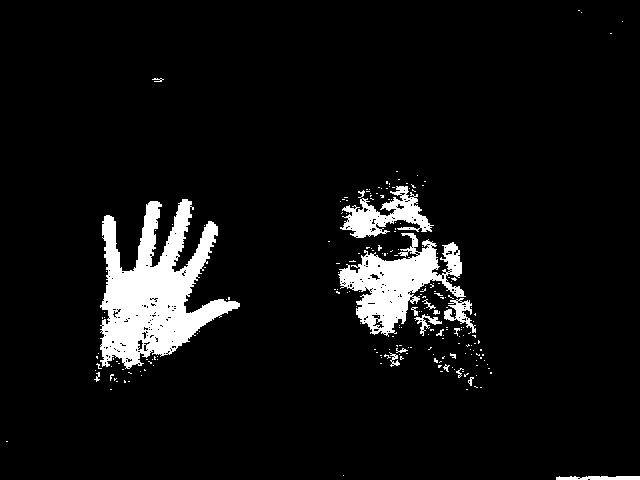
\includegraphics[width=0.9\columnwidth]{bilder/whiteskin}
  \caption{Figuren visar de områden i bilden som klassats som hud.
  Observera det vita bruset i bildens kanter, vilket filtreras bort med
  morfologiska operationer.}
  \label{fig:hudklassificering}
\end{figure}

\begin{figure}
  \centering
  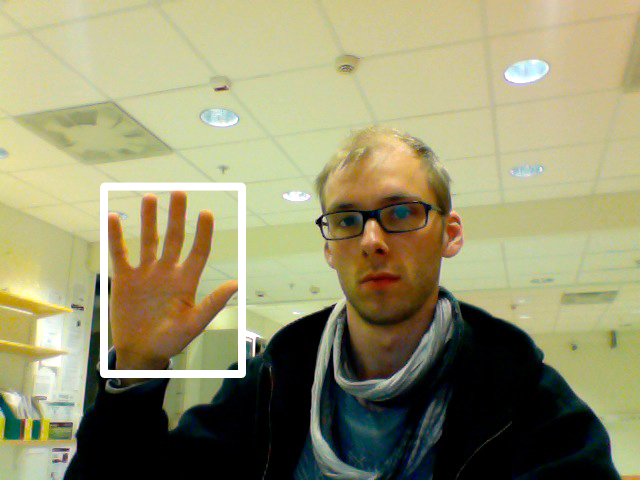
\includegraphics[width=0.9\columnwidth]{bilder/boundingbox}
  \caption{Handen har ringats in av programmet, som det
  ''tillräckligt'' stora objekt som befinner sig
  längst till vänster i bilden.}
  \label{fig:boundingbox}
\end{figure}

\end{document}
